\documentclass[conference]{IEEEtran}
\usepackage{graphicx,cite,url}
\renewcommand{\ttdefault}{lmtt}
\pdfinfo{/Author (RISC-V CPU) /Creator () /Producer () /Title (5-Stage Pipelined RISC-V Processor)}
\newcommand{\phaseTwoReport}{}
\title{5-Stage Pipelined RISC-V Processor}
\author{\IEEEauthorblockN{Aryan Kinha, Preetish Ubhrani, Divyanshu Singh,\\Jatin Kumar Singh, Jatin Verma}
\IEEEauthorblockA{Newton School of Technology, Rishihood University}}
\begin{document}
\raggedbottom
\maketitle

\begin{abstract}
We implemented a five-stage RISC-V processor in Verilog and compared it with a single-cycle core that executes the same instruction subset. The pipeline forwards results to EX, stalls for one cycle on an immediate load dependency, and clears two younger slots on a taken branch. Three unpadded benchmarks check arithmetic dependencies, load-use dependencies, and a loop with both branch outcomes. Both cores match the same instruction-by-instruction model. On a routed Lattice iCE40HX8K implementation using the branch benchmark ROM, the pipeline reached an estimated 42.74 MHz and the single-cycle core reached 30.37 MHz. Pipeline fill, stalls, and taken branches increased the cycle count enough that the single-cycle core still had the lower estimated completion time on that workload.
\end{abstract}
\begin{IEEEkeywords}
RISC-V, Verilog, pipelining, forwarding, load-use interlock, FPGA
\end{IEEEkeywords}

\section{Literature Review}
The RISC-V unprivileged specification defines what each instruction does to architectural state and how it is encoded~\cite{isa}. The implementation can split those operations across cycles as long as the program observes the required behavior. We used the same instruction semantics for the pipeline, the single-cycle baseline, and the software model.

In a single-cycle datapath, fetch, decode, execution, memory access and write-back all fit between two active clock edges. The longest path fixes the clock period. In a multi-cycle datapath, one instruction can take several cycles. Splitting it into steps gives the designer a chance to reuse hardware at the cost of control state and intermediate registers~\cite{patterson}. Pipelining also splits the work, but overlaps successive instructions. It can improve throughput even when one instruction takes multiple cycles to complete~\cite{harris}.

Overlap creates three common hazards. A structural hazard occurs when two stages need the same resource, such as a single memory port shared by fetch and load/store. Separate memories avoid that conflict here. A data hazard occurs when an instruction needs a value from an earlier instruction. A bypass can supply a result from a later stage, and an interlock can hold the consumer when the value is still being read from memory. Instructions in this design read and write registers in order, so read-after-write dependencies are the ones that need handling. A control hazard occurs when fetch runs ahead of a branch decision. Prediction, earlier resolution, and flushing are common responses~\cite{patterson,harris}.

PicoRV32 shows how a small core can expose a simple memory interface and make register-file design choices independently of the ISA~\cite{pico}. Ibex couples a configurable core with a larger verification effort~\cite{ibex}. VexRiscv offers configurable bypass and interlock behavior~\cite{vex}, whereas CV32E40P is an in-order pipeline with its own prescribed timing and interfaces~\cite{cv}. Our prototype keeps fixed stage boundaries and local memories. The student \texttt{risc-5-processor} project illustrates the use of an instruction model and repeatable randomized tests to check a processor alongside directed cases~\cite{comparison}. We use those checks to find errors that can disappear from the final machine state after later writes.

\section{Proposed Solution}
\subsection{Instruction subset and memory}
Both cores support the operations in Table~\ref{tab:enc} using standard RV32I encodings. NOP is ADDI x0,x0,0. Arithmetic wraps at the word width. The immediate decoder sign-extends I, S and B immediates, with the implicit low zero bit restored for branch offsets. The decoder validates the opcode and function fields before enabling architectural effects.

\begin{table}[t]
\caption{Supported encodings. Fields are in hexadecimal.}
\label{tab:enc}
\centering
\begin{tabular}{lcccc}\hline
Instruction & Format & Opcode & funct3 & funct7\\\hline
ADD  & R & 33 & 0 & 00\\
SUB  & R & 33 & 0 & 20\\
ADDI & I & 13 & 0 & --\\
LW   & I & 03 & 2 & --\\
SW   & S & 23 & 2 & --\\
BEQ  & B & 63 & 0 & --\\
BNE  & B & 63 & 1 & --\\\hline
\end{tabular}
\end{table}

The memories hold 64 words each. The PC and effective addresses are byte addresses, and a word access requires four-byte alignment. The instruction ROM loads a hex file. An out-of-range or unaligned instruction fetch returns NOP. An invalid data read returns zero and an invalid store leaves memory as it was. The subset omits architectural traps and byte/halfword operations. Synchronous active-high reset sets the PC to zero and clears writable state. Reads of x0 always return zero.

\subsection{Pipeline and control}
Fig.~\ref{fig:block} shows the stage boundaries. IF fetches from the PC and normally advances by four. ID reads the source registers and decodes the instruction. EX selects operands, computes the arithmetic result or effective address, and checks the branch condition. MEM reads or writes data memory, and WB chooses between the ALU result and memory data. The four pipeline registers carry the instruction PC, instruction word and validity along with the fields needed downstream. A bubble clears validity and side effects. The retirement interface exposes the completed instruction's PC, word and register write for the checker.

\begin{figure*}[t]
\centering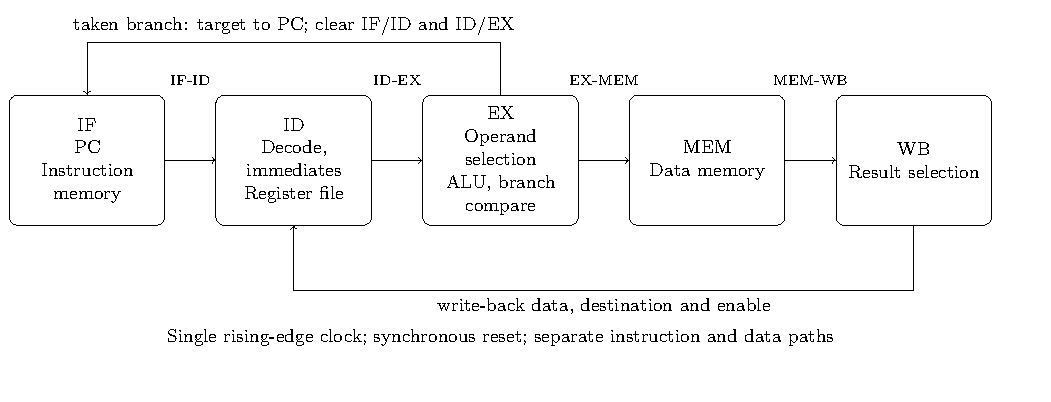
\includegraphics[width=\textwidth]{../diagrams/block.pdf}
\caption{Base datapath showing stage registers, the write-back path, and branch redirection. Forwarding feeds the EX operands. The interlock holds IF and ID and inserts a bubble into EX.}
\label{fig:block}
\end{figure*}

\begin{table}[t]
\caption{Decode control bits}
\label{tab:ctrl}
\centering\small
\begin{tabular}{lccccccc}\hline
 & RW & MR & MW & Imm & Sub & Br & NE\\\hline
ADD  &1&0&0&0&0&0&0\\
SUB  &1&0&0&0&1&0&0\\
ADDI &1&0&0&1&0&0&0\\
LW   &1&1&0&1&0&0&0\\
SW   &0&0&1&1&0&0&0\\
BEQ  &0&0&0&0&0&1&0\\
BNE  &0&0&0&0&0&1&1\\\hline
\end{tabular}
\par\smallskip\footnotesize RW: register write. MR/MW: memory read/write. Imm: use the immediate as ALU operand B. Sub: subtract. Br: branch. NE: compare for inequality.
\end{table}

Table~\ref{tab:ctrl} lists the control bits. The load bit also selects memory data in WB. Register and memory writes require a valid instruction. Each branch compares both source operands and adds the signed offset to its saved PC. On a taken branch, EX directs IF to the target and clears IF/ID and ID/EX at the next edge. The branch itself advances to MEM. The instruction in ID and the sequential fetch are discarded, with a cost of two slots.

\begin{figure*}[t]
\centering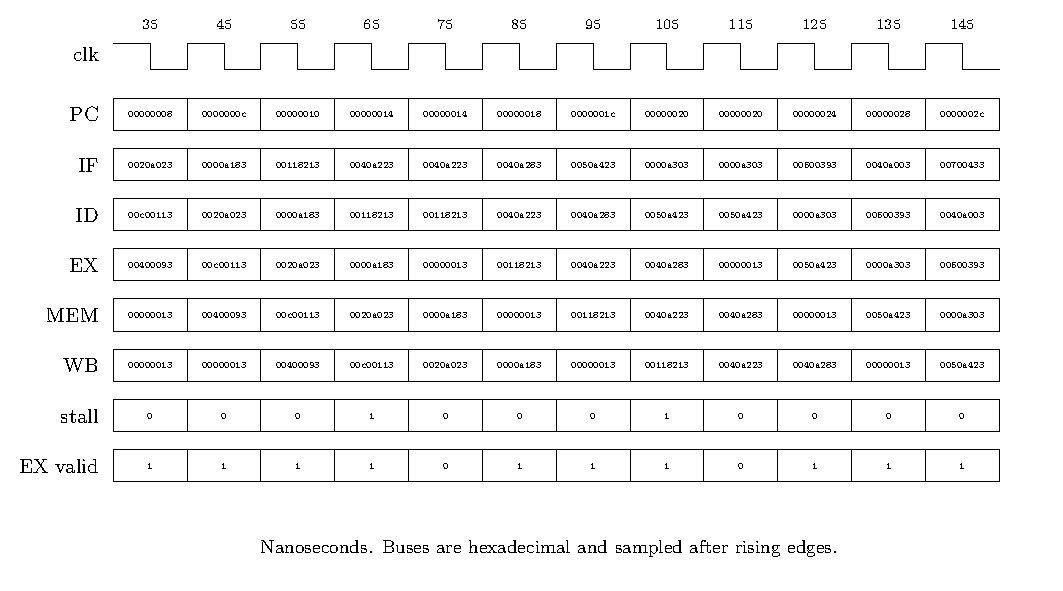
\includegraphics[width=\textwidth]{../waveforms/load_use.pdf}
\caption{Load-use VCD from the pipeline run. At 65 ns the load for x3 is in EX and its dependent ADDI is in ID. The edge at 75 ns holds the PC and ID and inserts a bubble. At 85 ns the ADDI enters EX as the load reaches WB. The visible second stall has a store-data dependency.}
\label{fig:wave}
\end{figure*}

\subsection{Forwarding and the load-use interlock}
Each EX source first checks for a valid, nonzero destination in EX/MEM. A matching ALU result there takes priority over one in MEM/WB because EX/MEM holds the more recent instruction. An EX/MEM load cannot forward its effective address as a register result. Its read data becomes available in MEM/WB, where WB supplies it to the consumer. The register file also passes a same-edge WB write to an ID read of that destination.

Forwarded A serves as the register operand for both arithmetic and address calculation. Forwarded B goes to the ALU on register-register operations, to the branch comparison, or to the store-data input. For a store the immediate still goes to the ALU for address calculation. This distinction matters when a load supplies the store value instead of its address.

The interlock checks a valid load in EX against a valid consumer in ID. Every supported instruction uses rs1. Only ADD, SUB, SW, BEQ and BNE use rs2, so an immediate that happens to share those bit positions cannot cause a false stall. The check also ignores loads to x0. On a match, the next edge holds the PC and IF/ID and inserts an invalid entry into ID/EX. The load advances. One cycle later the consumer enters EX and receives the value from WB. Reset and taken-branch redirection have priority over a hold.

\subsection{Single-cycle baseline}
The baseline uses the same decoder, ALU, memory modules and write-back selection. It has no interstage registers, so the current instruction reads register state left by preceding edges and writes its own result at the end of the cycle. Its register file disables same-cycle write-through. Enabling it on this datapath could feed an instruction's result back into its own source. A taken branch selects the target for the next fetch within the current cycle.

\section{Results and Discussion}
\subsection{Simulation and retirement checks}
Both cores were simulated with Icarus Verilog~\cite{icarus}. The ALU, register file and decoder pass 59 unit cases. The program suite checks 22 pipeline runs and three baseline runs. These include the four Phase I programs, three directed edge cases, twelve repeatable unpadded random programs, and three benchmark binaries run on both cores. GNU RISC-V binutils assembled the benchmark source. A separate instruction model checks the retired PC, instruction and register write in order. The benches also compare all 32 register entries and 64 data words against the expected final state.

The pipeline bench checks for simultaneous occupancy of all five stages at different instruction addresses. It also checks that a taken branch reaches the target and clears the two younger entries, and that a load-use stall holds fetch and decode while creating an EX bubble. In temporary copies, disabling one EX forwarding input or disabling the load interlock caused register-state failures. The complete suite passed from a fresh copy, and both RTL tops passed Verilator lint.

An instruction retires at its completion edge. This is WB in the pipeline and the end of the instruction's only cycle in the baseline. Valid stores, branches and explicit NOPs count, even when they write no register. A bubble or flushed instruction does not count. Each bench counts from the first rising edge after reset release through retirement of the program's last instruction. The stop address is supplied to the bench. The cores continue fetching after this address.

\subsection{Benchmark cycle counts}
Table~\ref{tab:bench} uses identical binaries and stop addresses on both cores. CPI is cycles divided by retired instructions. IPC uses the reciprocal. The single-cycle results are 1.000 CPI and 1.000 IPC throughout. Each pipeline run satisfies
\[
C = N + 4 + S + 2T ,
\]
where $N$ is the number of retirements, $S$ is the number of stalls and $T$ is the number of taken branches. The four-cycle term is pipeline fill before the first retirement.

\begin{table}[!t]
\caption{Cycle counts and pipeline CPI/IPC from RTL simulation. Both cores retire the same instruction sequence.}
\label{tab:bench}\centering\footnotesize
\setlength{\tabcolsep}{2.3pt}
\begin{tabular}{lrrrrrrr}\hline
 & & \multicolumn{2}{c}{Cycles} & & & \multicolumn{2}{c}{Pipeline}\\
Benchmark & Ret. & Single & Pipe & Stalls & Taken & CPI & IPC\\\hline
ALU chain   &  7 &  7 & 11 & 0 & 0 & 1.571 & 0.636\\
Load use    & 14 & 14 & 21 & 3 & 0 & 1.500 & 0.667\\
Branch loop & 18 & 18 & 31 & 1 & 4 & 1.722 & 0.581\\\hline
\end{tabular}
\end{table}

The ALU chain incurs no stalls even though consecutive instructions reuse results, including two successive writes to x1. The load benchmark stalls once for each of three immediate load dependencies. Fig.~\ref{fig:wave} shows a load followed by dependent arithmetic and another load followed by a store that uses its value. An independent ADDI and a load to x0 cause no stalls. The loop has three taken backward branches and one taken forward branch after a load. A skipped store and a skipped register write test that clearing the younger slots prevents wrong-path effects. The short, fixed programs make the sources of extra cycles easy to see. They do not estimate CPI for a general workload.

\subsection{Synthesis and FPGA timing}
We synthesized both tops with Yosys 0.71+77 and placed and routed them with nextpnr-ice40 (revision 15b77f5f)~\cite{fpga}. Both use the branch-loop ROM, the same externally visible fetch and retirement signals, the same iCE40HX8K CT256 device, seed~1 and a 12 MHz clock target. Table~\ref{tab:fpga} records the final routed estimates. Tool logs and JSON reports are reproduced by the repository's FPGA script.

\begin{table}[t]
\caption{Post-route utilization and clock estimates}
\label{tab:fpga}\centering
\begin{tabular}{lrr}\hline
Metric & Single-cycle & Pipeline\\\hline
Logic cells & 5,310 & 5,843\\
Block RAMs & 0 & 0\\
I/O pins & 169 & 169\\
Maximum clock (MHz) & 30.37 & 42.74\\\hline
\end{tabular}
\end{table}

The pipeline uses more logic cells, and its estimated maximum clock is about 1.41 times the baseline's. The local arrays use combinational reads, and writable state is cleared synchronously. This build maps the memories to logic. The wide debug outputs also occupy package pins, so the utilization describes these measured tops.

At their separate estimated maximum clocks, the branch benchmark takes about 0.593 microseconds on the single-cycle core ($18/30.37$) and 0.725 microseconds on the pipeline ($31/42.74$). The corresponding throughput estimates are 30.37 and 24.82 million retirements per second for the measured interval. At the shared 12 MHz target, completion time follows cycle count directly. These results describe the routed benchmark image and automatic pin placement. They do not include board-level I/O timing or measurements on physical hardware.

\section{Individual Contributions}
The module ownership below follows the repository contributions. Aryan Kinha coordinated integration and verification as team lead.

\begin{center}\footnotesize
\begin{tabular}{p{0.36\columnwidth}p{0.54\columnwidth}}\hline
Member & Module ownership\\\hline
Aryan Kinha\newline 2401020013 & Top-level integration, tests and report.\\
Preetish Ubhrani\newline 2401020050 & Execute stage, ALU and branch comparison.\\
Divyanshu Singh\newline 2401010161 & Decode, control, immediates and register file.\\
Jatin Verma\newline 2401010200 & Data memory, MEM/WB and write-back.\\
Jatin Kumar Singh\newline 2401010199 & Fetch, PC, instruction memory and IF/ID.\\\hline
\end{tabular}
\end{center}

\section{Conclusion}
The five-stage core executes the tested instruction sequences without software padding. Forwarding handles adjacent ALU dependencies, and the interlock covers loads that cannot produce data in time for the next EX stage. The two cores agree on the architectural effects checked by the reference model. The routed pipeline has a shorter estimated clock period, while the extra cycles in the measured branch loop outweigh that gain. The comparison is limited to the supported instructions, benchmark images and FPGA target described here.

\begin{thebibliography}{10}
\bibitem{isa} RISC-V International, \emph{The RISC-V Instruction Set Manual, Volume I: Unprivileged Architecture}, ver. 20240411, 2024. [Online]. Available: \url{https://docs.riscv.org/reference/isa/v20240411/unpriv/unpriv-index.html}
\bibitem{patterson} D. A. Patterson and J. L. Hennessy, \emph{Computer Organization and Design RISC-V Edition: The Hardware Software Interface}, 2nd ed. Morgan Kaufmann, 2020. [Online]. Available: \url{https://shop.elsevier.com/books/computer-organization-and-design-risc-v-edition/patterson/978-0-12-820331-6}
\bibitem{harris} S. L. Harris and D. Harris, \emph{Digital Design and Computer Architecture, RISC-V Edition}. Morgan Kaufmann, 2021. [Online]. Available: \url{https://pages.hmc.edu/harris/ddca/ddcarv.html}
\bibitem{pico} YosysHQ, ``PicoRV32: A size-optimized RISC-V CPU,'' source repository. Accessed: Nov. 13, 2026. [Online]. Available: \url{https://github.com/YosysHQ/picorv32}
\bibitem{ibex} lowRISC, ``Ibex RISC-V core,'' source repository. Accessed: Nov. 13, 2026. [Online]. Available: \url{https://github.com/lowRISC/ibex}
\bibitem{vex} SpinalHDL, ``VexRiscv,'' source repository. Accessed: Nov. 13, 2026. [Online]. Available: \url{https://github.com/SpinalHDL/VexRiscv}
\bibitem{cv} OpenHW Group, ``CORE-V CV32E40P RISC-V IP,'' source repository. Accessed: Nov. 13, 2026. [Online]. Available: \url{https://github.com/openhwfoundation/cv32e40p}
\bibitem{icarus} Icarus Verilog contributors, ``Icarus Verilog documentation.'' Accessed: Nov. 13, 2026. [Online]. Available: \url{https://steveicarus.github.io/iverilog/}
\bibitem{comparison} Ario2006, ``risc-5-processor,'' source repository, revision 6a9a36c. Accessed: Nov. 15, 2026. [Online]. Available: \url{https://github.com/Ario2006/risc-5-processor/tree/6a9a36c8434b05719c9045d768cd16f4a9162eca}
\ifdefined\phaseTwoReport
\bibitem{fpga} D. Shah, E. Hung, C. Wolf, S. Bazanski, D. Gisselquist, and M. Milanovi\'{c}, \textquotedblleft Yosys+nextpnr: An open source framework from Verilog to bitstream for commercial FPGAs,\textquotedblright\ in \emph{Proc. IEEE 27th Annu. Int. Symp. Field-Programmable Custom Computing Machines (FCCM)}, 2019, doi: 10.1109/FCCM.2019.00010.
\fi
\end{thebibliography}

\end{document}
